\section{Cultivation and differentiation of HAoSMCs}
\label{sec:cultivation}
For the following experiments \acp{haosmc} were used. A cell type commonly used for the study of cardiovascular function and disease [Reference for this claim]. Cells were kept at 37°C and 5\% CO2 when ever possibile.\\
Cells were differentiated treated first with \ac{tgf} and then with \ac{il1} \& \ac{pdgf} to induce a synthetic phenotype. For more imformation please check the section \ref{sec:haosms} on smooth muscle cells in \ac{cad}.

    \subsection{Thawing \& Cultivation}
    Cells were cultivated to a maximum passage of 10, after that new passage cells were thawed. For long time storage cells were kept in [cryo medium] and stored in liquid nitrogen. When required, new cells (6th passage) were need cells were thawed at 37°C in the water bath and transfered to a falcon. After centrifugation for 2 min at 300xg the supernatant was removed and the cell pellet taken up in 14 mL of M231 + \ac{smgs} for cultivation in a T75 flask. Every other day 2/3 of the medium were removed and replaced by fresh.

    \subsection{Passaging}
    When reaching a maximum of ~80\% confluency (approx. once a week) the medium was removed completely and cells were washed once with 5 mL of \ac{pbs}. Then the cells were incubation with 3 mL trypsin for 4 min at 37°C. After 7 mL M231 were added to the deattched cells and the cells were transfered to a falcon and pelleted for 4 min at 300xg. The supernatant was removed and the pellet resuspended in M231 + SMGS, seeding ~$\num{500e3}$ cells per T75 flask.

    \subsection{Preparation of Collagen I matrix}
    For preparation of the \ac{col1} matrix (1.8 mg/mL) all the components were mixed, adding the collagen last. All components were stored at 4°C and all pipetting steps were carried out on ice:

    \begin{table}[h]
    \capstart
	\centering
	\begin{minipage}{\captionwidth}
	   	\caption[Col I matrix]{\uzlemph{\ac{col1} Matrix Composition}}
	   	\label{tab:qPCR_samples}
	\end{minipage}
    \begin{tabular}{|c|c|c|}
        \hline
        component & concentration & volume (µL) \\ \hline
        H20       & -             & 38.9        \\
        M231      & -             & 53.3        \\
        SMGS      & 20x           & 5,3         \\
        NaOH      & 1 M           & 2,7         \\
        NaHCO3    & 7.5 \%        & 2.1         \\
        Col I     & 5 mg/mL       & 57.6        \\ \hline
        total     & -             & 160         \\ \hline
    \end{tabular}
    \end{table}

    160 µL of matrix mix were transfered in each used well of a 24-well plate, fully coating the bottom of the well. For polymerization the matrix was incubated at 37°C for at least 60 min.

    \subsection{Differentitation of HAoSMCs}
    Differentiation was carried out in 24 wells plates with 1 mL M231 supplemented with 1 \% \ac{fbs} and different cytokines:
    \begin{itemize}
        \item \textbf{Day 0:} Matrix and cells were prepareed as described in the sections Preparation of \ac{col1} matrix and Passaging. Seeding of $\num{40e3}$ in M231 + \ac{smgs} on plastic or on 160 µL \ac{col1} matrix.
        \item \textbf{Day 1:} After ~24 h the medium was replaced with 1 mL M231 + 1\% \ac{fbs} + 5 ng/mL \ac{tgf} (or just 1 mL M231 + 1\% \ac{fbs}).
        \item \textbf{Day 5:} The medium was replaced with 1 mL M231 + 1\% \ac{fbs} + 10 ng/mL \ac{il1} + 10 ng/mL \ac{pdgf} (or just 1 mL M231 + 1\% \ac{fbs}).
        \item \textbf{Day 7:} Potentially further stimulation described in the section of the used assay.
    \end{itemize}

\section{mRNA Quantification}
\label{sec:qpcr}
\ac{qpcr} was utilized to assess the m\ac{rna} concentration of the two reporter genes \ac{cnn1} and \ac{mmp9} in \acp{haosmc} differentiated as described in section on differentiation. Using the house keeping gene \ac{gapdh} for reference.\\
SYBR® Green is an intercalating \ac{dna} dye that allows for the monitoring of \ac{dna} amplification. Flourescence is measured after every amplification cycle of the PCR yielding a crossing point when signal reaches a certain threshhold. A lower \ac{Cq} corresponds to an higher inital \ac{dna} concentration \cite{huggettStandardisationReportingNucleic2011}.

    \subsection{\ac{rna} Isolation}
    \ac{rna} was isolated using the kit and extraction was performed according to the corresponding protocol, using an extra washing step with 700 µL 80 \% ethanol and eluting with 30 µL of RNase-free water. Determination of nucleic acid concentration was carried out with the NanoDrop.

    \subsection{Reverse Transcription}
    For \ac{RT}, \ac{rna} samples were diluted to yield 10 µL of ~ 10 ng/µL \ac{rna}. The samples were heated for 5 min at 68°C before adding 10 µL of the RT reaction mix described in the following table:

    \begin{table}[h]
    \capstart
	\centering
	\begin{minipage}{\captionwidth}
	   	\caption[RT mastermix]{\uzlemph{RT Master Mix}}
	   	\label{tab:RT Mastr Mix}
	\end{minipage}
    \begin{tabular}{|c|c|c|}
        \hline
        component           & concentration & volume (µL) \\ \hline
        First Strand Buffer & 5x            & 4           \\
        \acs{DTT}            &               & 2           \\
        \acs{dNTP}           &               & 1           \\
        Oligos              &               & 1           \\
        RiboLock            &               & 1           \\
        M-MLVRT             &               & 1           \\ \hline
    \end{tabular}
    \end{table}

    The reaction was carried out for 60 min at 37°C before inactivating the enzyme for 5 min at 95°C. cDNA was used for qPCR or stored at -20°C.

    \subsection{qPCR}
    The samples were prepared in a 384-well plate using SYBR® Green Master Mix:

    \begin{table}[h]
    \capstart
	\centering
	\begin{minipage}{\captionwidth}
	   	\caption[qPCR samples]{\uzlemph{qPCR samples}\newline The samples for the qPCR}
	   	\label{tab:qPCR_samples}
	\end{minipage}
    \begin{tabular}{|c|c|c|}
        \hline
        component                  & conentration & volume (µL) \\ \hline
        SYBR GREEN Master Mix      & 1:2          & 3.75        \\
        Primer (forward + reverse) & 5 pM (each)  & 1.125       \\
        H20                        & -            & 1.125       \\
        cDNA                       & -            & 1.5           \\ \hline
    \end{tabular}
    \end{table}

    Wells were sealed, thoroughly mixed by invertation of the plate and the assay performed using follwing programme on the TaqMan:

    \begin{table}[h]
    \capstart
    \centering
    \begin{minipage}{\captionwidth}
        \caption[qPCR programme]{\uzlemph{qPCR programme}\newline The programme for the qPCR}
        \label{tab:qPCR_programme}
    \end{minipage}
    \begin{tabular}{|c|c|c|c|c|}
    \hline
        step & time (s) & temperature (°C) & loop to & passes \\ \hline
        1    & 120      & 50               &         & 1      \\
        2    & 600      & 95               &         & 1      \\
        3    & 15       & 60               &         & 40     \\
        4    & 60       & 60               & 3       & 40     \\
        5    & 600      & 95               &         & 1      \\
        6    & -        & 16               &         & 1      \\ \hline
    \end{tabular}
    \end{table}

    \subsection{Processing of Data}
    The Cq was automatically calculated by the software SDS2.2.2 and exported for further analysis. The arithmetic  mean of three 3 technical was calculated for each sample, disregarding values that are obvious outliers. For normalization the mean ct of the reference gene GAPDH was substracted from the mean ct of the gene of interest:

    $$\Delta ct = ct(\mathrm{gene of interest}) - ct(\mathrm{GAPDH})$$

    Taking into account the exponential amplification of DNA in PCR, the $\Delta ct$ can then be transformed into an relative expression level. Where $\num{10e6}$ is just a constant to yield values that are easier to work with:

    $$\mathrm{rel. expr.} = 2^{-\Delta ct\num{10e6}}$$

    In total four biological replicates were done. Data visualization and statistical analysis was done in python using the modules: pandas, numpy, scipy as well as pyplot and seaborn. Assuming a normal distribution, student's t-test was used, a p-value of 0.05 is considered as significant. For detailed information please check the script.

\section{Energy Profiling}
\label{sec:seahorse}
Seahorse Assay was utilized to assess the energy profile of HAoSMC differentiated as described in section on differentiation. For this assay cells were not differentiated in a 24 well plate but the seahorse plate, using 5 technical repeats and on control well for 4 tested conditions. Since the plate would not fit the matrix cells were cultivated in plastic!\\
The Seahorse XF Analyzer allows real time measurement of dissolved oxygen and protons in a confined small volume by using solid state sensor probes. These are used to calculate the oxygen consumption rate (OCR) and extracellular acidification rate (ECAR) of a cell monolayer. The OCR and ECAR are indicators for mitochondrial respiration and glycolisis respectively and can be used to assess the metabolic function of cells \cite{HowAgilentSeahorse}.

    \subsection{Seahorse Assay}
    On the day before the assay the Seahorse XF Analyzer was turned on to calibrate and the sensor cartrigae was left to equilibrate in Seahorse XF calibrant over night at 37 °C (in non-CO2 environment).\\
    On the day of the assay, cells were washed with 500 µL PBS each and afterwards 500 µL supplemented XF BASE medium were added, cells were left to incubate for 1 h at 37°C in non-CO2 environment. During this time toxins for disruption of the respiratory chain were prepared and added to the catridge:

    \begin{table}[h]
    \capstart
    \centering
    \begin{minipage}{\captionwidth}
        \caption[toxins for seahorse]{\uzlemph{toxins for seahorse}\newline toxins for seahorse. :)}
        \label{tab:seahorse_toxins}
    \end{minipage}
    \begin{tabular}{|c|c|c|c|}
        \hline
        component  & concentration in cartridge(µM) & volume in cartridge(µL) & concentration in well (µM) \\ \hline
        Oligomycin & 14                             & 55                      & 1.4                        \\
        FCCP       & 10                             & 60                      & 2.0                        \\
        Antimycin  & 50                             & 65                      & 5.0                        \\ \hline
    \end{tabular}
    \end{table}

    The compound catridge was loaded into the XF Analyser for calibration, after successful calibration the hydration catridge was replaced with the cell plate. Measurement was carried out as following:

    \begin{itemize}
        \item Calibration of the probes.
        \item Equilibration
        \item 3 Repeats of:
        \begin{itemize}
            \item Mixing (1 min)
            \item Pause (2 min)
            \item Detection of OCR and EACR (4 min)
        \end{itemize}
        \item Pause (2 min)
        \item Injection of 55 µL Oligomycin
        \item 3 Repeats of:
        \begin{itemize}
            \item Mixing (1 min)
            \item Pause (2 min)
            \item Detection of OCR and EACR (4 min)
        \end{itemize}
        \item Pause (2 min)
        \item Injection of 60 µL FCCP
        \begin{itemize}
            \item Mixing (1 min)
            \item Pause (2 min)
            \item Detection of OCR and EACR (4 min)
        \end{itemize}
        \item Pause (2 min)
        \item Injection of 55 µL Antimycin
        \item 3 Repeats of:
        \begin{itemize}
            \item Mixing (1 min)
            \item Pause (2 min)
            \item Detection of OCR and EACR (4 min)
        \end{itemize}
    \end{itemize}

    Finally the medium was removed and cells were stained for 15 min with Hoechst (concentration in PBS) and photographed in the keyence to determine cell count for normalization.

    \subsection{Processing of Data}
    Cells were quantified using (what exactly does Tobias script do) with a python script provided by my supervisor Dr. Tobias Reinberger, cell count and the signal of the control wells were used to normalize the OCR and EACR calculated by the XF Analyzer with the accompanying software.\\
    In total three biological were recorded of which on was excluded because no changes in OCR and EACR could be detected and cells deacttched from the bottom of the wells during Hoechst staining. For the remaining two replicates the least fitting of the 5 technical repeats for each condition was manually excluded.\\
    Further , again using a modified python script provided by Dr. Tobias Reinberger. Assuming a normal distribution, student's t-test was used, a p-value of 0.05 is considered as significant. For detailed information please check the script.

\section{Oxidative Stress Assay}
\label{sec:cellrox}
CellROX Green assay was used to assess generation of reactive oxygen species in HAoSMC differentiated as described in section on differentiation, after further stimulation (from here on refered to as 'boost') with PDGF. Additionally a recovery experiment was performed using NAC, a potent anioxidant, to quench generation of ROS.

\noindent CellROX Green is a flourescent dye that gets oxidized by ROS and then binds to DNA, showing bright green flourescence \cite{CellROXGreenReagent}.

    \subsection{CellROX Assay}
    For the assay cells were washed with PBS then the boost was performed using variable concentrations of PDGF in 300 µL HBSS. For ROS quenching with NAC, 0.25 M NAC solution was added to the wells 2 h prior to the experient and also added to HBSS during the experiment.

    \begin{table}[h]
    \capstart
    \centering
    \begin{minipage}{\captionwidth}
        \caption[Seahorse Assay]{\uzlemph{Seahorse Assay}}
        \label{tab:cellrox_table}
    \end{minipage}
    \begin{tabular}{|c|c|c|c|}
        \hline
        component         & concentration & final concentration      & volume (µL) \\ \hline
        HBSS              & -             & -                        & 300         \\
        PDGF              & ?             & variable (0 - 400 ng/mL) & variable    \\
        Hoechst           & ?             & ?                        & 0.3         \\
        CellROX   (1:500) & ?             & ?                        & 0.6         \\
        NAC               & 0.25 M        & variable (0 - 8 mM)      & variable    \\ \hline
        total             & -             & -                        & $\sim$300   \\ \hline
    \end{tabular}
    \end{table}

    Cells further kept at 37°C in 5 \% CO2 environment, incubation time is indicated with the results of the respective experiment. Imaging was done at the keyence microscope using standard sensitivity and a exposure time of s in the green channel and s for the blue channel.

    \subsection{Processing of Data}
    For time resolved PDGF-BB boost titration 7 biological repeats were performed of which one was excluded because of high signal in the negative control. For NAC quench 4 biological repeats were performed of which one was excluded because no signal in the positive control.\\
    For quantification of signal itensity, pixels with a green value higher than 90 were counted. Differents in cell count were adjusted by divison by the number of pixels with a blue value bigger than 80 (CHECK TRESHHOLD VALUES!!). Z-STACK FOR THE NAC quench images. To adjust for large variance in total signal intensity between biological repeats, values were adjusted by divison through the total signal of all recorded conditions.\\
    Mann Whitney U Test was used, a p-value of 0.05 is considered as significant. For detailed information please check the scripts.


\section{Immunoflourescence}
\label{sec:if}
Fibronektion as marker of matrix. Used cells.
Maybe also the anti-8-oxoG AB?

    \subsection{Protocol}
    First cells were washed with PBS and fixated for 40 min with 200 µL -20°C methanol-aceton (1:1), after the removal of methanol-aceton cells were left to dry for 20 min. Then cells were treated for 30 min with 250 µL permeabilization buffer, folllowed by 30 min with 250 µL blocking buffer and incubated with 300 µL of the primary AB over night at 4°C:

    The next day the primary AB was removed and cells wre incubated for 60 min at RT with the secondary AB:

    After removal of the secondary AB cells were washed 3 times with PBS and stained for 15 min with DAPI (1:5000 in water).

    \subsection{Processing of Data}
    Me counting pixels.

\section{Curation of Data for postGWAS Analyses}
\label{sec:database}
GWAS data and data for postGWAS analyses and co-visualization was downloaded from public resources. Processing of the data and further annotation is briefly described in the follwing listing. For a complete overview of all the data collected please refer to table or the download scripts. For explainaition of the data please refer to the introdcution or the sources themselves.

\begin{itemize}
    \item \uzlemph{GWAS Summary Statistics:} The CAD GWAS summary statistics as well as a list of indetified proxy SNPs from the study was annotated with [what did Tobias do] via the ensembl REST API by Dr. Tobias Reinberger.
    \item \uzlemph{HGNC Gene List} The newest quarterly update to the complete HGNC dataset was downloaded via the FTP server. The dataset was used to generate a list of all approved symbols, mapping to their HGNC id. Further a list of all symbols (approved, alias and previous) was generated, mapping to their HGNC id.
    \item \uzlemph{Linked SNPs} LD $r^2$ values for variants in a 500 kb window around all variants in the list of CAD GWAS proxy variants, were computed and downloaded via the ensembl REST API. For humans ensembl calculates the LD with data from the 1000 Genomes project (see table). In the same process linked SNPs were annotated with their most severe consequence (by VEP) via the ensembl REST API.
    \begin{table}[h]
    \capstart
    \centering
    \begin{minipage}{\captionwidth}
        \caption[1000 Genomes Populations]{\uzlemph{1000 Genomes Populations}}
        \label{tab:populations}
    \end{minipage}
    \begin{tabular}{|c|c|c|}
        \hline
        Name                   & Size (individuals)   & Description      \\ \hline
        1000GENOMES:phase3:ALL & 2504                 & All phase 3 individuals  \\
        1000GENOMES:phase3:AMR & 347                  & Americans  \\
        1000GENOMES:phase3:EAS & 504                  & East Asians  \\
        1000GENOMES:phase3:EUR & 503                  & European \\
        1000GENOMES:phase3:SAS & 489                  & South Asian  \\ \hline
    \end{tabular}
    \end{table}
    \item \uzlemph{Ensembl Genome Annotatation} The newest ensembl build (ensembl release 106) was downloaded via the FTP server. Features annotated as genes of the type protein coding, lncRNA or miRNA were extracted, further gene symbols were mapped to their HGNC id if possible.
    \item \uzlemph{Open Target Genetics l2g Scores} The lattest list of Open Target Genetics l2g Scores was downloaded via the FTP server. Entrie were annotated with their HGNC ID when ever possible, entries that do not map to a gene that is approved by the HGNC were dropped.
    \item \uzlemph{Ensembl Regulatory Build} The newest ensembl regulatory build (ensembl release 106) was downloaded via the FTP server.
    \item \uzlemph{TSS} Transcription start sides for protein coding genes were extracted from a USCS Brower dump.
    \item \uzlemph{Associated traits from GWAS catalog} The SNP trait associations from the lattest release of the GWAS catalog as well as the accompanying list of studies was downloaded via the FTP server. SNP-trait correlations missing a the position or a p-value for the association were dropped from the data set. Further the column for Odds Ration or beta was seperated in to two columns.
    \item \uzlemph{TADs} The data on TAD was downloaded via the download link on the 3D genome browser.
    \item \uzlemph{scATAC-seq from Miller et al.} The processed scATAC seq data was scraped from the Miller Lab GitHub repository.
    \item \uzlemph{scATAC-seq from CATlas} The processed scATAC seq data was scraped from the Ren Lab website.
    \item \uzlemph{ABC model} The ABC model data was downloaded from the Engreitz Lab FTP server. The data was translated from Hg19 to Hg38 with pyliftover.
    \item \uzlemph{ENCODE cCREs} Done by Dr. Tobias Reinberger.
\end{itemize}


\section{Visualization of GWAS data}
\label{sec:gwas_vis}
For visualization of the data, an bokeh application was build, that fetches the data from the database and renders it to a webbrowser.\\
Bokeh is a python module that allow easy and interactive visualization of data. It combines the powerful data processing tools of python with the interactivity of JavaScript running in the browser. The python side of bokeh creates python objects which are serialized into JSON data and handed over to bokehJS which deserializes them into JavaScript objects that are rendered to the browser. The intergrated bokeh server additionally offers the possiblity to synchronize data between the underlying python environment and brower side JavaScript library, allowing real time updates to the displayed data.

    \begin{figure}[h]
    \capstart
        \centering
    	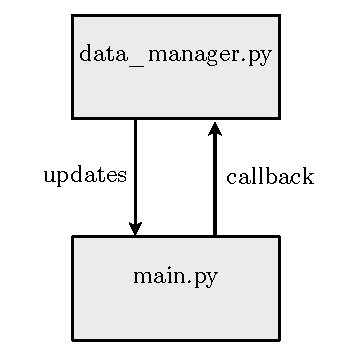
\includegraphics{Abbildung/vis_architecture.pdf}

    	\begin{minipage}{\captionwidth}
    		\caption[vis archi]{\uzlemph{Architecture of the vis tool} \newline }
    		\label{fig:db}
    	\end{minipage}
    \end{figure}

According to good design principles the concerns of the application are split into two sections. Reading of data from the database and further processing steps are managed by a data provide and enclosed in one class. In contrast to the model-controler-view architecture, a popular architectural pattern for the design of user interfaces, there is no partition between a view and a controler. Since data visualization as well as the control widgets are created by bokeh, it is convienient to use the build in event listeners of the library to handle the required callbacks. Therefore the main file is responsilbe for the creation of all plots and widgets as well as listening for inputs.

STYLING USING A bootstrap thingy

\section{Enrichment analysis}
\label{sec:enrichment}
Based in the data in the database initial postGWAS studies were run. Annotation enrichment analyses are a popular tool for the identification of terms that are over-represent in a list of interest. The most prominent application probably being their application as gene set enrichment analyses (GESA). GESA are used to check for the over-representtion of a candidate gene list in a predefined set of genes \cite{tipneyIntroductionEffectiveUse2010}. In this case the method is used to determine if regulatory elements which overlap with SNPs associated with CAD are enriched in a biosample, using fisher's exact test.\\
As a list of regulatory elements the cell type specific cCREs that are part of the ENCODE project were used (excluding cCREs marked as unclassified). As a list of SNPs the list of CAD associated proxy SNPS and linked variants (european population, r2 >= 0.6) was used. The four values required for calculation of the enrichment factor () and p-value require are shown in the Contingency of figure:

\begin{itemize}
    \item Number of distinct cCREs among all biosamples (m)
    \item Number of distinct cCREs that are annotated in the biosample of interest (mt)
    \item Number of distinct cCREs that overlap with a SNP in the SNP list in any biosample (n)
    \item Number of distinct cCREs that overlap with a SNP in the SNP list in the biosample of interest (nt)
\end{itemize}

\begin{figure}[h]
\capstart
    \centering
    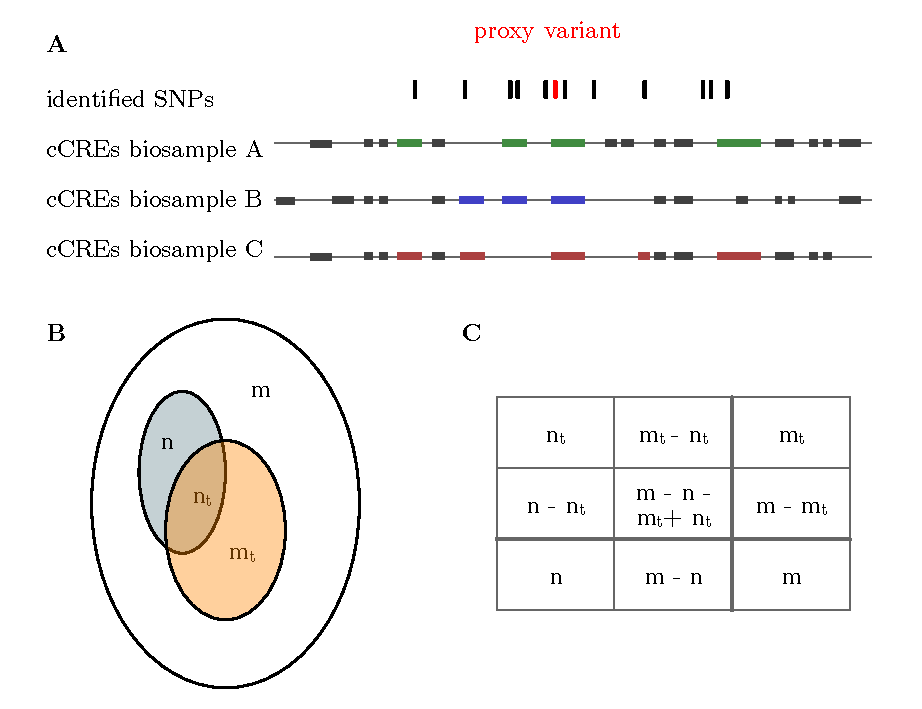
\includegraphics{Abbildung/enrichment.pdf}

    \begin{minipage}{\captionwidth}
        \caption[enrichment]{\uzlemph{enrichment}}
        \label{fig:enrichment}
    \end{minipage}
\end{figure}

The p-value for the number of overlaps to be greater than or equal to the observation can be calculated as the cumulative distribution function of the hypergeometric distribution.

$$ P(\sigma_t\geq n_t) = \sum_{k=n_t}^{min(m_t, n)} \frac{\binom{n}{k}\binom{m-n}{m_t-k}}{\binom{m}{m_t}} $$

To account for the multiple comparisons problem, p-values were adjusted with Bonferroni correction where n is the number of tests ($\equiv$ number of biosamples):

$$ p_{ajd.} = p*n$$

The analysis and visualization were done in python. A p-value of 0.05 is considered as significant. For detailed information please check the analysis script and the visualization script.
